% ===============================================================
%  Prever para Planear — artigo científico
%  Formato: Springer Lecture Notes in Computer Science (llncs.cls)
%
%  Compilação:  ./build.sh
%          ou:  latexmk -pdf -outdir=build artigo.tex
%          ou:  no Overleaf, carregar esta pasta e escolher artigo.tex
%               como documento principal
%
%  Limite: 12 páginas, referências incluídas.
% ===============================================================

\documentclass[runningheads,a4paper]{llncs}

% ---------------------------------------------------------------
% metadados.tex
% Editar APENAS este ficheiro para mudar o título, os autores e a
% afiliação do artigo.
% ---------------------------------------------------------------

\newcommand{\tituloprincipal}{Prever para Planear: Integração de Modelos de
  Aprendizagem Automática na Evasão Preditiva de Obstáculos em Veículos
  Autónomos}

% Título curto, usado no cabeçalho das páginas ímpares.
\newcommand{\titulocurto}{Prever para Planear}

% ---------------------------------------------------------------
% Autoria
%
% TODO: confirmar os elementos do grupo. A lista abaixo foi copiada do
% relatório de ENGCIA (repo projeto-1); apagar ou acrescentar linhas
% conforme o grupo deste trabalho. Os autores separam-se com \and.
% ---------------------------------------------------------------
\newcommand{\listaautores}{%
  Ana Salomé Ferreira Teixeira \and
  Diogo Miguel Gonçalves Ribeiro \and
  João Gabriel Domingos de Azevedo \and
  Pedro Nuno Verde Cerqueira \and
  Rúben Alexandre Abreu Freitas \and
  Rúben Carlos Zamith Ribeiro%
}

% Autores no cabeçalho das páginas pares (forma abreviada).
\newcommand{\autorescurtos}{A. Teixeira et al.}

% Nomes usados nos metadados do PDF (propriedades do ficheiro).
\newcommand{\autoresmeta}{%
  Ana Salomé Ferreira Teixeira;
  Diogo Miguel Gonçalves Ribeiro;
  João Gabriel Domingos de Azevedo;
  Pedro Nuno Verde Cerqueira;
  Rúben Alexandre Abreu Freitas;
  Rúben Carlos Zamith Ribeiro%
}

% ---------------------------------------------------------------
% Afiliação e contactos
% ---------------------------------------------------------------
\newcommand{\instituicao}{Instituto Superior de Engenharia do Porto (ISEP),
  Politécnico do Porto}
\newcommand{\curso}{Mestrado em Engenharia de Inteligência Artificial}
\newcommand{\morada}{Rua Dr.\ António Bernardino de Almeida 431,
  4249-015 Porto, Portugal}
\newcommand{\emails}{\{1210803, 1260429, 1211519, 1260443, 1231267,
  1161532\}@isep.ipp.pt}

% ---------------------------------------------------------------
% Palavras-chave (separadas por \and)
% ---------------------------------------------------------------
\newcommand{\palavraschave}{Condução autónoma \and Previsão de trajetórias
  \and Aprendizagem automática clássica \and Planeamento de movimento
  \and A* \and Waymo Open Motion Dataset}

% ---------------------------------------------------------------
% preambulo.tex — pacotes, estilos e macros
%
% A classe llncs (Springer LNCS) define as margens, os tipos de letra e
% os títulos. Não se alteram aqui: mexer em margens ou tamanhos de letra
% faz o artigo deixar de cumprir o formato (e o limite de páginas).
% ---------------------------------------------------------------

\usepackage[T1]{fontenc}
\usepackage[utf8]{inputenc}
% Português. Com o ficheiro de língua clássico (portuges.ldf) usa-se esse;
% numa instalação mínima sem ele, o babel moderno carrega a língua pelo
% ficheiro .ini. O resultado é o mesmo.
% O babel clássico torna " um atalho que «come» o carácter seguinte;
% desativa-se, para que aspas escritas diretamente não estraguem o texto.
\IfFileExists{portuges.ldf}%
  {\usepackage[portuguese]{babel}%
   \AtBeginDocument{\shorthandoff{"}}}%
  {\usepackage[portuguese,provide=*]{babel}}
\usepackage{lmodern}       % Computer Modern em T1 (acentos nativos)
\usepackage{microtype}

\usepackage{graphicx}
\usepackage{booktabs}
\usepackage{amsmath}
\usepackage{amssymb}
\usepackage{icomma}        % vírgula decimal em modo matemático: $1,5$
\usepackage{xcolor}
\usepackage{tikz}          % diagrama da arquitetura
\usetikzlibrary{positioning,arrows.meta}

% --- Cores -------------------------------------------------------
\definecolor{corEscura}{HTML}{1F3A5F}
\definecolor{corAviso}{HTML}{B45309}

% --- Ligações ----------------------------------------------------
\usepackage[pdfusetitle]{hyperref}
\hypersetup{
  colorlinks=true,
  linkcolor=corEscura,
  citecolor=corEscura,
  urlcolor=corEscura
}
% URL e DOI das referências no tipo de letra do texto (recomendação da
% Springer), em vez de monoespaçado.
\renewcommand\UrlFont{\rmfamily}

% O cleveref não traz nomes em português; definem-se aqui.
\usepackage[capitalise,noabbrev,nameinlink]{cleveref}
\crefname{section}{Secção}{Secções}
\crefname{subsection}{Secção}{Secções}
\crefname{figure}{Figura}{Figuras}
\crefname{table}{Tabela}{Tabelas}
\crefname{equation}{Equação}{Equações}
\newcommand{\crefrangeconjunction}{ a }
\newcommand{\crefpairconjunction}{ e }
\newcommand{\crefmiddleconjunction}{, }
\newcommand{\creflastconjunction}{ e }

% --- Textos fixos da classe llncs em português -------------------
% O babel traduz «Resumo», «Figura», «Tabela» e «Referências»; as
% palavras-chave são da classe e traduzem-se à mão.
\AtBeginDocument{%
  \renewcommand{\keywordname}{\textbf{Palavras-chave:}}%
  \renewcommand{\andname}{e}%            entre dois autores
  \renewcommand{\lastandname}{\unskip\ e}% antes do último autor
}

% --- Macros próprias ---------------------------------------------
% Informação em falta, realçada a laranja. Antes de entregar não pode
% sobrar nenhuma (o build.sh não as deteta: procurar por \preencher).
\newcommand{\preencher}[1]{\textcolor{corAviso}{\textbf{[#1]}}}

% Unidades com espaço fino e sem quebra de linha: \un{2,5}{m}.
\newcommand{\un}[2]{#1\,\mbox{#2}}

% Nomes de variáveis do código (colunas das tabelas de dados).
\newcommand{\var}[1]{\texttt{\detokenize{#1}}}


\begin{document}

\title{\tituloprincipal}
\titlerunning{\titulocurto}
\author{\listaautores}
\authorrunning{\autorescurtos}
\institute{\instituicao\\
  \curso\\
  \morada\\
  \email{\emails}}

\maketitle

% Resumo: 150 a 250 palavras (regra do formato LNCS).
\begin{abstract}
Um veículo autónomo tem de prever o movimento dos outros utentes da via e
de usar essa previsão para planear o seu próprio movimento. Este artigo
revê o estado da arte nas duas frentes, a previsão de trajetórias e o
planeamento de movimento, e na forma como se ligam e se avaliam, com
atenção ao que conseguem os modelos de aprendizagem automática clássica,
sem redes neuronais. Apresenta ainda resultados preliminares de uma
arquitetura «prever para planear» sobre o Waymo Open Motion Dataset:
florestas aleatórias que aprendem, no referencial de cada veículo, a
correção a uma extrapolação de velocidade constante, e um planeador de
velocidade A* que trata as previsões como obstáculos móveis. Em 149 cenas
reais (13\,856 amostras, validação cruzada agrupada por cena), o erro
médio de posição desce de \un{4,97}{m} para \un{2,47}{m} a \un{3}{s} e de
\un{12,57}{m} para \un{6,66}{m} a \un{5}{s}, face à velocidade constante.
No planeamento, a versão atual do planeador ainda não converte esse ganho
numa redução mensurável dos conflitos; identificam-se as causas e o
trabalho necessário para o conseguir.

\keywords{\palavraschave}
\end{abstract}


% ~1 página
\section{Introdução}
\label{sec:introducao}

Os sistemas de condução autónoma organizam-se, em geral, numa cadeia de
módulos: perceção, previsão do movimento dos outros utentes da via,
planeamento e controlo~\cite{paden2016survey,schwarting2018planning}. A
previsão e o planeamento dependem um do outro. Um plano só é seguro se
contar com o sítio onde os outros veículos vão estar nos segundos
seguintes, e esse futuro não é conhecido: tem de ser estimado a partir do
que se observou até ao momento.

Este trabalho junta as duas metades do problema. Na previsão, a questão é
quanto se ganha com modelos de aprendizagem automática clássica (árvores
de decisão, florestas aleatórias, \emph{gradient boosting}) em relação às
extrapolações físicas mais simples. A restrição a modelos clássicos é
deliberada: treinam-se em segundos num computador comum, funcionam com
poucos dados e deixam ver que variáveis pesam na previsão. No
planeamento, a questão é se uma previsão melhor dá um plano melhor,
quando as previsões entram como obstáculos móveis num planeador de
velocidade baseado em pesquisa A*.

Os dados são os do Waymo Open Motion Dataset
(WOMD)~\cite{ettinger2021large}, que regista trajetórias reais de
veículos, peões e ciclistas em meio urbano. A escolha do problema foi
condicionada pelo que os dados permitem. Cada cena dura cerca de
\un{20}{s}, o veículo da Waymo percorre nela \un{96}{m} (mediana) e, em
82\% das cenas analisadas, há um único caminho possível entre o ponto de
partida e o de chegada. Não há pedidos de viagem nem frotas. Problemas de
rotas longas ou de despacho de veículos exigiriam dados inventados; as
interações locais entre veículos, pelo contrário, estão presentes em
todas as cenas.

O artigo tem três contributos:
\begin{itemize}
  \item uma revisão do estado da arte em previsão de trajetórias, em
    planeamento de movimento e na ligação entre os dois
    (\cref{sec:estado-arte});
  \item uma arquitetura «prever para planear» com modelos clássicos e um
    planeador A* (\cref{sec:abordagem});
  \item resultados preliminares em 149 cenas reais, com as limitações que
    ainda têm (\cref{sec:resultados}).
\end{itemize}

% ~5,5 páginas — é a secção principal do artigo.
\section{Estado da arte}
\label{sec:estado-arte}

% ---------------------------------------------------------------
\subsection{Dados e métricas de previsão}
\label{sec:dados-metricas}

A investigação em previsão de movimento apoia-se em conjuntos de dados
públicos. O WOMD~\cite{ettinger2021large} tem mais de 100\,000 cenas de
\un{20}{s}, num total de 574 horas a \un{10}{Hz}, com as trajetórias de
veículos, peões e ciclistas e o mapa da zona. A tarefa oficial dá
\un{1}{s} de passado e pede os \un{8}{s} seguintes. O
Argoverse~\cite{chang2019argoverse} tem 324\,557 sequências de \un{5}{s},
com \un{2}{s} observados e \un{3}{s} a prever, e distingue-se por
publicar, ao lado dos modelos neuronais, referências que não o são:
velocidade constante e regressão por vizinhos mais próximos. Em
autoestrada, o highD~\cite{krajewski2018highd} reúne trajetórias
recolhidas por \emph{drone}.

As métricas habituais medem distâncias entre a trajetória prevista e a
real~\cite{chang2019argoverse,ettinger2021large}. O erro médio de
deslocamento (ADE) é a média dessa distância ao longo do horizonte; o
erro final (FDE) é a distância no último instante. Quando o modelo propõe
$K$ trajetórias, conta a melhor delas (minADE, minFDE), e a taxa de
falhas (\emph{miss rate}) é a fração de casos em que nenhuma fica perto do
ponto final real (a menos de \un{2}{m}, no Argoverse). Neste trabalho
prevê-se uma única trajetória por veículo, pelo que a métrica é o FDE.

% ---------------------------------------------------------------
\subsection{Previsão de movimento}
\label{sec:previsao}

A classificação mais citada separa os modelos em três níveis: os físicos,
que só usam a dinâmica do veículo; os baseados em manobras, que primeiro
reconhecem a intenção do condutor; e os que consideram a interação entre
veículos~\cite{lefevre2014survey}. Uma revisão mais recente organiza os
métodos pela técnica: modelos físicos, aprendizagem automática clássica,
aprendizagem profunda e aprendizagem por
reforço~\cite{huang2022survey}. É a segunda família que este trabalho
explora.

\paragraph{Modelos físicos.}
Assumem que o veículo mantém a velocidade, a aceleração ou a taxa de
viragem que tem no momento. São os modelos usados no seguimento de
veículos com filtros de Kalman, contexto em que foram
comparados~\cite{schubert2008comparison}. Não precisam de treino,
mas só são fiáveis a muito curto prazo, abaixo de um
segundo~\cite{lefevre2014survey}: ignoram a estrada, os semáforos e os
outros veículos.

Ainda assim, são referências difíceis de bater, e por isso qualquer
modelo aprendido deve ser comparado com elas. Na previsão de peões, a
velocidade constante superou modelos neuronais do estado da arte nos
conjuntos de dados habituais~\cite{scholler2020constant}. Para veículos,
a \cref{tab:baselines} reúne valores publicados. A distância para os
modelos aprendidos cresce com o horizonte, e no WOMD a velocidade
constante erra mais de \un{5}{m} logo aos \un{3}{s}.

\begin{table}[t]
\centering
\caption{Erros publicados da velocidade constante e de modelos aprendidos
  na previsão de veículos, em metros, com uma trajetória proposta por
  veículo, exceto onde se indica $K$.}
\label{tab:baselines}
\begin{tabular*}{\textwidth}{@{\extracolsep{\fill}}llllll@{}}
\toprule
Dados & Horizonte & Métrica & Vel.\ const. & Modelo aprendido & Fonte \\
\midrule
Argoverse & \un{3}{s} & minFDE & 7,89 & 4,97 (LSTM)
  & \cite{chang2019argoverse} \\
NGSIM & \un{3}{s} / \un{5}{s} & RMSE & 3,13 / 6,68
  & 2,09 / 4,37 (CS-LSTM) & \cite{deo2018convolutional} \\
WOMD & \un{3,1}{s} / \un{5,1}{s} & minFDE & 5,7 / 14,1 & --
  & \cite{munozsanchez2022scenario} \\
WOMD & \un{8}{s} & minADE & 11,0 & 1,34 (LSTM, $K{=}6$)
  & \cite{ettinger2021large} \\
\bottomrule
\end{tabular*}
\end{table}

\paragraph{Aprendizagem automática clássica.}
Antes das redes profundas, a previsão fazia-se com classificadores e
regressores sobre variáveis calculadas à mão. Máquinas de vetores de
suporte e modelos de Markov escondidos distinguiram condutores que cumprem
ou violam a sinalização em cruzamentos, com validação em dados de condução
real~\cite{aoude2012driver}. Em autoestrada, uma floresta aleatória
estima a probabilidade de cada manobra e uma regressão por misturas
gaussianas converte-a numa distribuição de
trajetórias~\cite{schlechtriemen2015when}. O estudo mais sistemático
nesta linha, com mais de 30\,000~km de dados de autoestrada, concluiu que
a floresta aleatória classifica as manobras melhor do que um perceptrão
multicamada e do que um classificador bayesiano ingénuo, e obteve um erro
lateral mediano inferior a \un{0,21}{m} a
\un{5}{s}~\cite{wirthmuller2021teaching}. O Argoverse dá o contraponto:
a regressão por vizinhos mais próximos, aplicada diretamente às
trajetórias passadas, fica ao nível da velocidade constante
(\un{7,88}{m} contra \un{7,89}{m} a
\un{3}{s})~\cite{chang2019argoverse}. O modelo, por si só, não chega; contam
as variáveis que recebe.

As florestas aleatórias~\cite{breiman2001random} e o \emph{gradient
boosting}~\cite{friedman2001greedy} são hoje os modelos de referência
para dados em tabela. Estes trabalhos concentram-se, porém, em classificar
manobras em contextos específicos, sobretudo a mudança de faixa em
autoestrada. Na pesquisa feita para este artigo não se encontrou nenhum
que aplique modelos clássicos à regressão de trajetórias no WOMD, em meio
urbano.

\paragraph{Aprendizagem profunda.}
Os melhores resultados atuais vêm de redes neuronais que recebem as
trajetórias e o mapa quase em bruto. A VectorNet representa faixas e
agentes como vetores ligados num grafo~\cite{gao2020vectornet}; o
Trajectron++ combina um grafo de agentes com redes recorrentes e garante
previsões dinamicamente possíveis~\cite{salzmann2020trajectron}; o Motion
Transformer, que liderou a tabela do WOMD, atinge um minFDE de
\un{1,22}{m} com seis trajetórias propostas, em média sobre os horizontes
de 3, 5 e \un{8}{s}~\cite{shi2022motion}. Estes números não se comparam
diretamente com os de uma previsão única. O preço é o volume de dados, o
treino em GPU e a dificuldade em explicar cada previsão.

\paragraph{Duas ideias que não dependem do modelo.}
A primeira é o referencial. Os modelos centrados no agente, que descrevem
a cena a partir da posição e da orientação do veículo a prever, são
invariantes a translações e rotações e dominam as tabelas
públicas~\cite{su2022narrowing,shi2022motion}. A segunda é aprender uma
correção em vez da trajetória inteira: parte-se da previsão de um modelo
baseado em conhecimento e o modelo aprendido estima apenas o resíduo, o
que melhora a exatidão e a generalização a cenas
novas~\cite{bahari2021injecting}. Ambas se aplicam a modelos clássicos e
são a base da abordagem da \cref{sec:abordagem}.

% ---------------------------------------------------------------
\subsection{Planeamento de movimento}
\label{sec:planeamento}

O planeamento divide-se habitualmente em níveis: a rota na rede viária, a
decisão de comportamento (seguir, ceder, mudar de faixa), o planeamento de
movimento, que produz uma trajetória, e o
controlo~\cite{paden2016survey}. No planeamento de movimento há três
grandes famílias: pesquisa em grafos, amostragem e otimização
numérica~\cite{paden2016survey}.

\paragraph{Pesquisa em grafos.}
O espaço de estados é discretizado e procura-se o caminho de menor custo.
O A* expande primeiro os estados com menor soma do custo já gasto com uma
estimativa do custo em falta; se essa heurística nunca sobrestimar, a
solução é ótima~\cite{hart1968formal}. Para lidar com obstáculos móveis, o
tempo e a velocidade passam a fazer parte do
estado~\cite{ziegler2009spatiotemporal}. A decisão longitudinal em meio
urbano foi formulada como planeamento discreto resolvido por A*, com uma
heurística construída a partir dos estados de colisão inevitável e um
pior caso de \un{80}{ms} para um horizonte de
\un{13}{s}~\cite{hubmann2016generic}. O trabalho mais próximo do aqui
proposto pesquisa sobre o tempo, a distância percorrida, a faixa e a
velocidade discreta, trata os outros veículos como obstáculos no
espaço-tempo, previstos com velocidade constante e uma margem de
segurança, e usa como heurística o custo de um problema
relaxado~\cite{ajanovic2018search}.

\paragraph{Decomposição caminho-velocidade.}
Uma simplificação clássica resolve o problema em dois passos: primeiro
um caminho que evita os obstáculos fixos, depois um perfil de velocidade
ao longo dele que evita os obstáculos móveis no plano distância-tempo
(S--T)~\cite{kant1986toward}. Em estrada, o caminho natural é o eixo da
faixa, e as trajetórias descrevem-se em coordenadas de Frenet (distância
ao longo da faixa e desvio lateral), onde se geram polinómios que
minimizam a variação da aceleração~\cite{werling2010optimal}. O planeador
EM do Apollo, de uso industrial, segue esta decomposição: otimiza o
caminho e a velocidade em separado, com programação dinâmica para uma
solução grosseira e programação quadrática para a
refinar~\cite{fan2018baidu}.

\paragraph{Regras e garantias.}
O Intelligent Driver Model (IDM) calcula a aceleração a partir da
distância e da velocidade relativa ao veículo da
frente~\cite{treiber2000congested}; é o modelo que controla os outros
veículos nos simuladores
atuais~\cite{karnchanachari2024towards,gulino2023waymax}. O modelo RSS define
formalmente as distâncias longitudinais e laterais que um veículo deve
manter para nunca ser responsável por um
acidente~\cite{shalevshwartz2017formal}, e pode fundamentar a margem de
segurança de um planeador.

% ---------------------------------------------------------------
\subsection{Da previsão ao planeamento}
\label{sec:integracao}

\paragraph{Formas de integração.}
Uma revisão recente distingue três: sequencial, em que a previsão é feita
primeiro e entra no planeador como dado de entrada ou termo de custo; não
dirigida, em que as duas tarefas são resolvidas em conjunto; e
bidirecional, em que o plano influencia a
previsão~\cite{hagedorn2025integration}. A abordagem deste trabalho é
sequencial. A sua limitação conhecida é tratar os outros como obstáculos
que não reagem, o que torna o veículo defensivo; modelar o efeito das
ações próprias nos outros condutores dá comportamentos mais
eficientes~\cite{sadigh2016planning}.

\paragraph{Uma previsão melhor dá um plano melhor?}
Não necessariamente. A exatidão medida em dados fixos não acompanha de
forma fiável o desempenho na condução, por duas razões: o plano do veículo
altera o comportamento dos outros, e um preditor mais pesado atrasa o
planeador~\cite{tran2023what}. As métricas de exatidão tratam todos os
erros por igual, quando só alguns mudam o plano, o que motivou métricas
que têm em conta o planeamento~\cite{ivanovic2022injecting}. O exemplo
mais forte é o PDM-Closed, um planeador por regras que prevê os outros
veículos com velocidade constante e escolhe entre propostas geradas pelo
IDM: no nuPlan obteve 92 e 93 pontos em simulação, contra 72 e 73 do
melhor planeador aprendido (com e sem veículos reativos), apesar de ter
a pior pontuação quando avaliado apenas contra o
registo~\cite{dauner2023parting}.

\paragraph{Como se avalia um planeador.}
Em ciclo aberto, compara-se o plano com o que o condutor real fez. Em
ciclo fechado, o plano é executado num simulador e o planeador volta a
decidir a cada passo. Os outros veículos podem repetir o registo, sem
reagir, ou ser controlados por um modelo reativo como o
IDM~\cite{karnchanachari2024towards}. O nuPlan mede colisões por culpa
própria, permanência na zona transitável, progresso, tempo até à colisão e
conforto~\cite{karnchanachari2024towards}; o Waymax oferece as mesmas
duas opções sobre as cenas do WOMD~\cite{gulino2023waymax}. A repetição
do registo tem um defeito conhecido: quando o plano se afasta do que
aconteceu, a simulação diverge e surgem colisões com veículos que, na
realidade, teriam reagido~\cite{karnchanachari2024towards,hagedorn2025integration}.

% ---------------------------------------------------------------
\subsection{Síntese}
\label{sec:sintese}

Da revisão saem três conclusões que orientam o resto do trabalho.
Primeiro, a velocidade constante é a referência obrigatória e o seu erro
no WOMD é conhecido (\cref{tab:baselines}). Segundo, os modelos clássicos
têm resultados sólidos na classificação de manobras em autoestrada, mas
não foram encontrados trabalhos que os usem para prever trajetórias no
WOMD. Terceiro, o ganho em exatidão só interessa se chegar ao plano, e
isso mede-se com o planeador, não com o erro de previsão. Tanto quanto
foi possível apurar, não existe uma comparação, com um planeador por
pesquisa sobre estes dados, entre quatro fontes de previsão: nenhuma,
velocidade constante, modelo clássico e futuro real.

% ~1,5 páginas
\section{Abordagem proposta}
\label{sec:abordagem}

A \cref{fig:arquitetura} resume a arquitetura. O código usa a biblioteca
scikit-learn~\cite{pedregosa2011scikit}.

\begin{figure}[t]
\centering
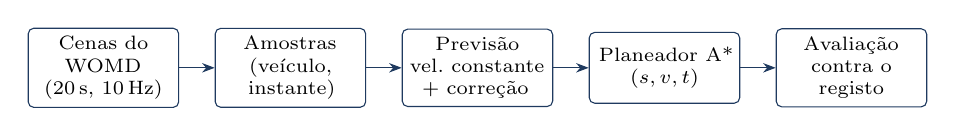
\begin{tikzpicture}[
    node distance=4.5mm,
    caixa/.style={draw=corEscura, rounded corners=2pt, align=center,
      font=\scriptsize, inner sep=3pt, minimum height=9mm, text width=17mm},
    seta/.style={-{Stealth[length=1.6mm]}, draw=corEscura}]
  \node[caixa] (dados) {Cenas do WOMD\\(\un{20}{s}, \un{10}{Hz})};
  \node[caixa, right=of dados] (amostras) {Amostras\\(veículo, instante)};
  \node[caixa, right=of amostras] (prev)
    {Previsão\\vel.\ constante\\+ correção};
  \node[caixa, right=of prev] (plan) {Planeador A*\\$(s, v, t)$};
  \node[caixa, right=of plan] (aval) {Avaliação\\contra o registo};
  \draw[seta] (dados) -- (amostras);
  \draw[seta] (amostras) -- (prev);
  \draw[seta] (prev) -- (plan);
  \draw[seta] (plan) -- (aval);
\end{tikzpicture}
\caption{Arquitetura «prever para planear»: das cenas gravadas ao plano de
  velocidade do veículo autónomo.}
\label{fig:arquitetura}
\end{figure}

\subsection{Dados e amostras}

Usam-se dois ficheiros da versão de \un{20}{s} do WOMD, com 149 cenas.
Uma amostra é um par (veículo, instante). Em cada cena toma-se um
instante por segundo e, nele, todos os veículos a menos de \un{55}{m} do
veículo autónomo, em movimento (pelo menos \un{0,5}{m/s}) e observados sem
falhas no segundo anterior. O resultado são 13\,856 amostras de 2\,343
veículos. O alvo é o deslocamento do veículo 1, 3 e \un{5}{s} depois; o
de \un{5}{s} só existe em 10\,295 amostras, porque muitos veículos deixam
de ser observados antes disso, e as restantes não entram no treino nem na
avaliação desse horizonte.

\subsection{Características e modelos}

Cada amostra é descrita por 21 variáveis calculadas apenas com o passado e
o presente, em três grupos:
\begin{itemize}
  \item movimento do próprio veículo, no seu referencial: velocidade
    longitudinal e lateral, aceleração estimada, taxa de viragem e
    deslocamento no último segundo;
  \item veículo da frente: distância, velocidade e velocidade de
    aproximação, quando existe um veículo ou ciclista na mesma direção, a
    menos de \un{60}{m} e de \un{1,8}{m} de desvio lateral (acontece em
    66\% das amostras);
  \item relação com o veículo autónomo: posição e velocidade relativas,
    distância, velocidade de aproximação e tempo até à colisão.
\end{itemize}

Seguindo as duas ideias da \cref{sec:previsao}, o modelo não prevê a
posição futura em coordenadas do mapa. Prevê, no referencial do veículo,
a diferença entre o deslocamento real e o que a velocidade constante
daria:
\begin{equation}
  \hat{\mathbf{d}}_h = \mathbf{v}\,h + f_h(\mathbf{x}),
  \qquad h \in \{1, 3, 5\}~\mathrm{s},
\end{equation}
em que $\mathbf{v}$ é a velocidade atual, $\mathbf{x}$ o vetor de
características e $f_h$ um modelo treinado para o horizonte $h$. Assim, um
veículo que segue em frente tem correção nula seja qual for a direção da
estrada no mapa, e o modelo concentra-se nos desvios: travagens,
acelerações e curvas. Comparam-se três modelos para $f_h$: árvore de
decisão (profundidade 6), floresta aleatória (60 árvores, profundidade 8)
e \emph{gradient boosting} por histogramas (80 iterações).

\subsection{Planeador}

O planeador segue a decomposição caminho-velocidade
(\cref{sec:planeamento}): o caminho é dado e planeia-se a velocidade. Um
estado é $(s, v, t)$, a distância percorrida, a velocidade e o instante,
com passo de \un{0,1}{s} e horizonte de \un{3}{s}. As ações são quatro
acelerações: $-3$, $-1,5$, $0$ e \un{$+1,5$}{m/s$^2$}. O custo de um plano
soma o desconforto (quadrado da aceleração) com uma penalização elevada
por cada passo a menos de \un{3,5}{m} da posição prevista de um veículo; a
heurística do A* premeia o progresso. As posições previstas vêm de uma de
quatro fontes: nenhuma (os outros ficam onde estão), velocidade constante,
floresta aleatória ou o futuro real, que serve de limite superior.

% ~1,5 páginas
\section{Resultados preliminares}
\label{sec:resultados}

Todos os valores desta secção vêm das 149 cenas descritas na
\cref{sec:abordagem} e de validação cruzada em cinco partes agrupada por
cena: nenhuma cena contribui ao mesmo tempo para o treino e para o teste.

\subsection{Previsão}

% A tabela sai de scripts/run_predict_to_plan.py (validação cruzada por cenário).

\begin{table}[t]
\centering
\caption{Erro final de posição (FDE), em metros: média e desvio-padrão
  das cinco partes da validação cruzada. «(mapa)»: posição prevista
  diretamente em coordenadas do mapa. Os três últimos modelos usam o
  referencial do veículo e a correção à velocidade constante.}
\label{tab:previsao}
\begin{tabular*}{\textwidth}{@{\extracolsep{\fill}}lccc@{}}
\toprule
Modelo & \un{1}{s} & \un{3}{s} & \un{5}{s} \\
\midrule
Velocidade constante & $0,68 \pm 0,02$ & $4,97 \pm 0,35$ & $12,57 \pm 0,90$ \\
Aceleração constante & $0,44 \pm 0,02$ & $3,32 \pm 0,12$ & $9,71 \pm 0,35$ \\
Floresta aleatória (mapa)
  & $0,89 \pm 0,10$ & $4,25 \pm 0,37$ & $10,02 \pm 0,73$ \\
\midrule
Árvore de decisão & $0,43 \pm 0,02$ & $2,78 \pm 0,14$ & $7,50 \pm 0,35$ \\
Floresta aleatória & $0,39 \pm 0,01$ & $2,47 \pm 0,12$ & $6,66 \pm 0,32$ \\
\emph{Gradient boosting} & $0,37 \pm 0,01$ & $2,36 \pm 0,10$ & $6,52 \pm 0,34$ \\
\bottomrule
\end{tabular*}
\end{table}

A \cref{tab:previsao} mostra três coisas. A velocidade constante erra
\un{4,97}{m} a \un{3}{s} e \un{12,57}{m} a \un{5}{s}, valores coerentes
com os \un{5,7}{m} e \un{14,1}{m} publicados para o mesmo conjunto de
dados em horizontes ligeiramente maiores (\cref{tab:baselines}). A
representação conta mais do que o modelo: a mesma floresta aleatória, a
prever a posição em coordenadas do mapa, perde para a aceleração
constante; no referencial do veículo e a prever a correção, reduz o erro
da velocidade constante para cerca de metade a 3 e a \un{5}{s}. E os três modelos clássicos ficam
próximos, com a floresta aleatória e o \emph{gradient boosting}
praticamente empatados.

As variáveis com mais peso na floresta aleatória são a aceleração
estimada (0,40), a taxa de viragem (0,15) e a velocidade de aproximação
ao veículo da frente (0,09). Sem as três variáveis do veículo da frente,
o erro a \un{3}{s} sobe de \un{2,47}{m} para \un{2,68}{m}. Treinar com
mais cenas quase não ajuda (\un{2,58}{m} com 25 cenas, \un{2,47}{m} com
119), o que indica que o próximo ganho virá de variáveis novas (mapa,
semáforos) e não de mais dados do mesmo tipo.

O mesmo conjunto de variáveis serve para classificar a manobra dos
\un{3}{s} seguintes em cinco classes (seguir em frente, acelerar, travar,
virar à esquerda, virar à direita). Numa divisão simples, com 37 cenas de
teste, a floresta aleatória acerta 75,6\% e o \emph{gradient boosting}
77,9\%; a classe mais frequente representa 55\% das amostras.

\subsection{Planeamento}

% Os valores da tabela e do texto saem de scripts/evaluate_planner_cv.py.

\begin{table}[t]
\centering
\caption{Planeador A* em 909 situações de 121 cenas, por fonte de
  previsão. Conflito: o plano passa a menos de \un{3,5}{m} da posição
  real de um veículo. Travagens máximas: passos de \un{0,1}{s} com a
  travagem mais forte, em média por situação. Intervalos de confiança a
  95\% por reamostragem das cenas.}
\label{tab:planeamento}
\begin{tabular*}{\textwidth}{@{\extracolsep{\fill}}lccc@{}}
\toprule
Previsão & Conflitos (\%) & Travagens máximas & Velocidade (m/s) \\
\midrule
Nenhuma & 21,8 [16,3; 27,3] & 0,11 & 5,49 \\
Velocidade constante & 20,7 [15,6; 25,7] & 0,02 & 5,38 \\
Floresta aleatória & 20,2 [15,1; 25,4] & 0,02 & 5,36 \\
Futuro real & 16,7 [12,0; 21,4] & 0,04 & 5,37 \\
\bottomrule
\end{tabular*}
\end{table}

A \cref{tab:planeamento} compara as quatro fontes de previsão. Cada
situação é um instante de uma cena com pelo menos um veículo à frente do
veículo autónomo, a menos de \un{25}{m}; em cada parte da validação
cruzada, a floresta é treinada nas outras quatro. Conhecer o futuro é
melhor do que qualquer das outras fontes: menos 3,5 a 5,1 pontos
percentuais de conflitos, com intervalos de confiança que excluem o zero.
Planear sem previsão distingue-se sobretudo pelas travagens máximas,
cinco vezes mais frequentes. Entre a velocidade constante e a floresta
aleatória a diferença é de 0,4 pontos percentuais, com intervalo de
confiança de $-0,8$ a $1,9$: não se distinguem. O ganho de exatidão da
\cref{tab:previsao} não chega, por agora, ao plano, o que está de acordo
com a literatura da \cref{sec:integracao}.

O valor do futuro real mostra onde está o problema: mesmo com previsões
perfeitas há conflitos em 16,7\% das situações, pelo que o limite está no
planeador e na avaliação, e não nas previsões. Há quatro causas
identificadas. O caminho é uma reta na direção atual do veículo, e não a
faixa. As posições dos outros veículos, previstas e reais, são
interpoladas em linha reta entre o instante atual e os \un{3}{s}. O
critério de conflito é uma distância entre centros, que conta veículos da
faixa do lado; em 3,7\% das situações já há um veículo a menos de
\un{3,5}{m} no instante inicial. E o teste executa um único plano de
\un{3}{s} em ciclo aberto, sem voltar a planear.

% ~0,5 página
\section{Conclusões e trabalho futuro}
\label{sec:conclusao}

A revisão mostra que as extrapolações físicas continuam a ser referências
fortes, que os modelos clássicos têm resultados sólidos em tarefas
específicas e que um erro de previsão menor não garante, por si só, um
plano melhor. Os resultados preliminares confirmam os dois lados. Com as
variáveis certas, uma floresta aleatória reduz para metade o erro da
velocidade constante a 3 e a \un{5}{s} em cenas urbanas reais. No
planeador atual, essa melhoria ainda não se traduz em menos conflitos.

O trabalho seguinte decorre das limitações identificadas:
\begin{itemize}
  \item planear ao longo da faixa, usando o mapa, com as previsões nos
    três horizontes em vez de uma interpolação;
  \item avaliar em ciclo fechado, voltando a planear a cada segundo, com
    um critério de colisão baseado nas dimensões dos veículos;
  \item acrescentar variáveis do mapa e dos semáforos à previsão;
  \item aumentar o número de cenas e separar treino e teste por local,
    porque o mesmo local aparece em várias cenas;
  \item comparar o A* com outras estratégias de pesquisa e medir o número
    de estados expandidos.
\end{itemize}


% Atribuição exigida pela licença do Waymo Open Dataset: tem de constar em
% qualquer trabalho feito com os dados. Não apagar.
\subsubsection*{Nota sobre os dados.}
Este trabalho foi feito com o Waymo Open Dataset, disponibilizado pela
Waymo LLC (\emph{made using the Waymo Open Dataset, provided by Waymo
LLC}), ao abrigo da licença para uso não comercial.


% Estilo de referências da Springer (numérico, com DOI). Só aparecem
% na lista as entradas de referencias.bib citadas no texto.
\bibliographystyle{splncs04}
\bibliography{referencias}

\end{document}
